\chapter{State of the Art}
\label{chapter:state_of_the_art}

This chapter aims to provide a description and overview of important concepts and protocols of \acf{bas}, \acf{iot} as well as event processing. For each topic there will be a review of the different technologies, how they interact and how they differ from each other.

All of the topics addressed in this chapter contributed to the solution presented, either in a combination of different technologies or choosing from similar ones.

\section{\acf{bas}}

A \acf{bas} consists in the automatic control and monitoring of building services such as lighting, heating, ventilation, air conditioning, and more. The main purpose of \ac{bas} is to improve the comfort of the building's occupants, while decreasing significantly the operational costs and energy consumption. This is achieved using the information gathered by a wide set of sensors, that is used to control building equipment behaviour such as lighting, \ac{hvac}, shutters, and others \cite{Brambley2005}. This information can also be used to prevent and react quickly to emergency situations, allowing to resolve them with minimum or even non human intervention.

\begin{figure}[H]
	\centering
	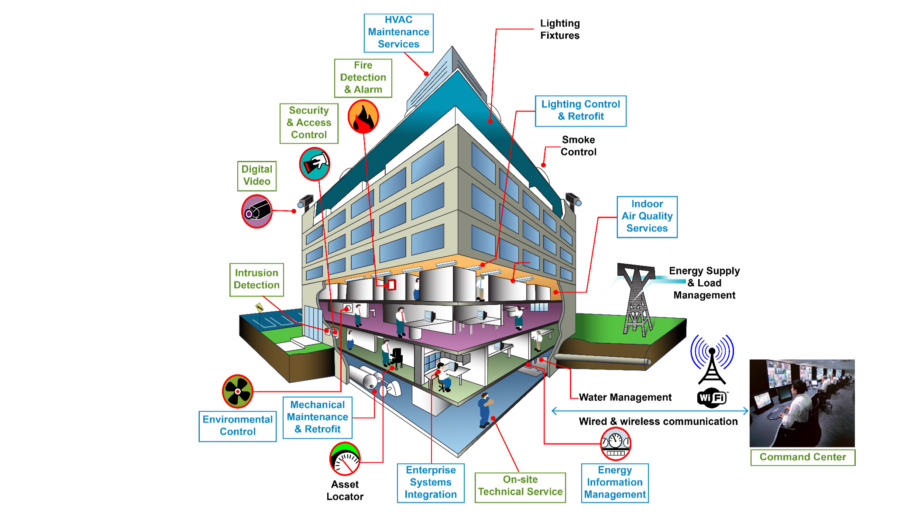
\includegraphics[width=0.9\textwidth]{figures/smart-building.jpg}
	\caption{Building Automation System schematic. Adapted from \cite{image-BAS}. }
	\label{fig:smart-building}
\end{figure}

The biggest problem in building automation is the market segmentation, where different manufactures created over the years different protocols and communication standards that didn't address solutions to all types of applications. This led to a more difficult and often impossible integration of this different approaches in the same system. Also, each vendor used to have closed specifications but, recently, in order to gain a higher margin of market, this specifications started being disclosed by vendors, which led to the appearence of new standards made from prior ones, combined. Presently the most used standards are BACnet, LonWorks, KNX and DALI. This different standards act in different \ac{bas} layers, which will be addressed in the next section. 

Though, with the rising of \ac{iot}, there have been an increasingly amount of new solutions that use high scalable technologies, well known communication standards, such as IP,  and use lightweight devices with low power consumption. This concepts will be addressed ahead in section 2.2.


\subsection{\ac{bas} Protocols}

In this section there will be addressed the most common technologies present at the current Building Automation market. Each one of them as an important role at different levels of a Building Automation System. As shown in Figure \ref{fig:hierarchy}, those levels are Management System Level, Automation Level and Field Level \cite{Iwayemi2011}. The all set of devices, sensors or actuators, compose the field layer. The Automation level is responsible for all the logic and hardware needed to control those devices and the Management Level consists in the control and management of the system and the reactions to events present in the gathered data.

\begin{figure}[H]
	\centering
	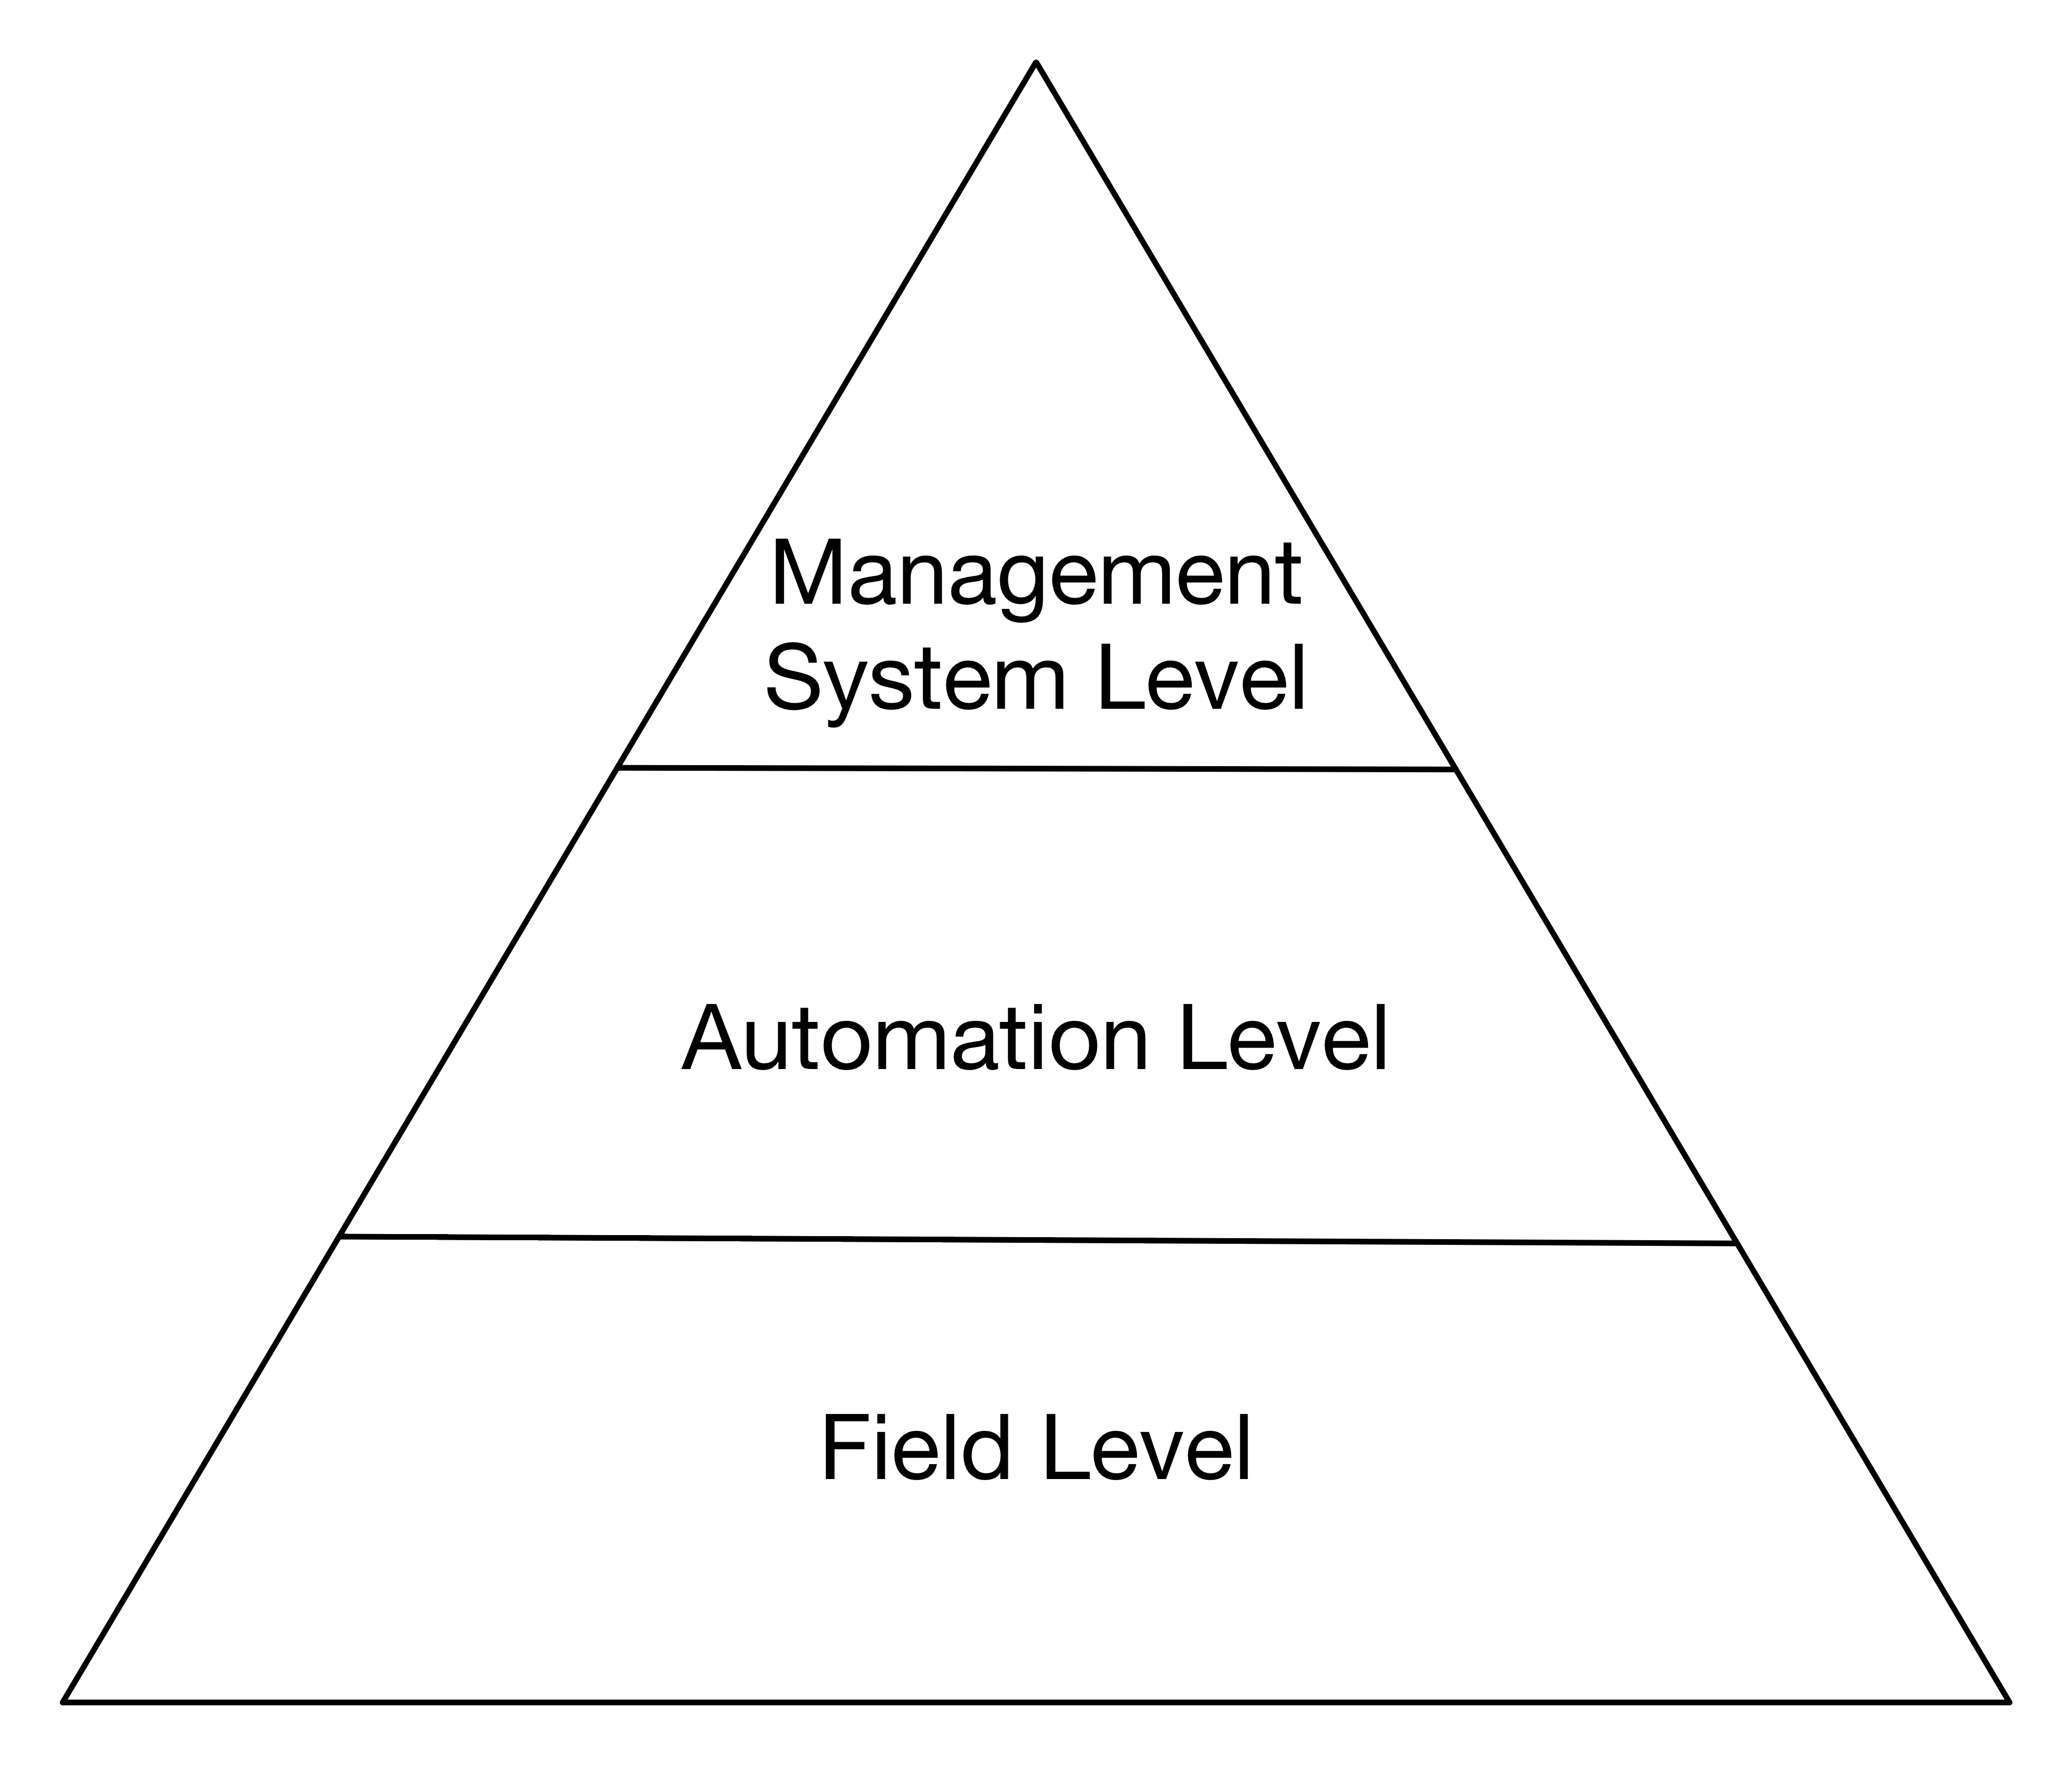
\includegraphics[width=0.9\textwidth]{figures/hierarchy.png}
	\caption{Building Automation System hierarchy \cite{kastener}. }
	\label{fig:hierarchy}
\end{figure}

The most common protocols used in BAS are \acf{bacnet} \cite{bacnet}, \acf{knx} \cite{knx}, \acf{lonworks} \cite{EchelonCorporation2009}, EnOcean \cite{enocean}, and \acf{dali} \cite{dali}. Each one of them has its own position on the \ac{bas} hierarchy. All the features of each one and the differences between them will be addressed in the next subsections.


\subsubsection{BACnet}
The \acf{bacnet} protocol, was developed by \acf{ashrae} in 1987 but was only published and accepted as a ANSI/ASHRAE standard latter in 1995.

\ac{bacnet} was designed to allow communication of building automation and control systems in fields such as HVAC, lighting control and others. The \ac{bacnet} protocol allow the deployment of automation mechanisms to sensors and actuators exchange information, irrespective of any service they perform.

\ac{bacnet} is modelled in object-oriented manner. There are a standard set object types that define the application services supported, such as devices, control loops, notifications, commands, schedules and more \cite{Domingues2016}. Each of the objects can have its own properties, that define together their functionality. For, example, a motion sensor can have multiple properties such as, number of times it was triggered and record of the last on-state time, and not only the current state. The access and manipulation of the object properties is done through a service that allows reading and writing object properties, that can interact with the real device state based on his object properties \cite{Fernbach2011}.

As stated before, other important \ac{bacnet} features are scheduling, which allow to schedule actions and program periodic events, notifications, that allow to distribute event notifications to the subscribed recipients \cite{Domingues2016} and logging, allowing a historical view of every change carried out in the system.

\ac{bacnet} is surely a complete solution that can be a good option for a full building automation system deployment. Yet \ac{bacnet} is an open standard, but the tools are supplied individually by each manufacturer \cite{openprotocol}, being sometimes complex the use and manage devices from different vendors. Figure \ref{fig:bacnet} shows an example of a multi vendor architecture.


\begin{figure}[H]
	\centering
	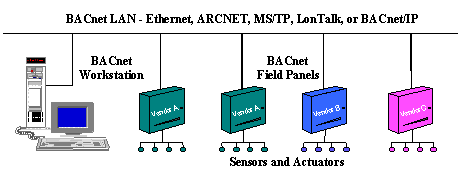
\includegraphics[width=0.9\textwidth]{figures/bacnet.png}
	\caption{Native BACnet architecture. Adapted from \cite{bacnetimage}. }
	\label{fig:bacnet}
\end{figure}


\subsubsection{KNX}

\ac{knx} was created from the combination of the best aspects of European Installation Bus (EIB), European Home Systems (EHS), and BatiBUS technologies. Later, KNX was standardized as norm EN 50090, and in 2006 as a international ISO/IEC 14543 standard \cite{Domingues2016}.

KNX deployment architecture uses a common bus connected to every device, actuator or sensor. The communication can be done using unicast addressing, since every device has a unique identifier corresponding to its position in the network. There is also the possibility of multicast communication since devices can be also aggregated in groups through a group identifier \cite{Kastner2005}.  

KNX support a variety of communication means such as twisted-pair (TP), power line (PL), IP tunnelling and a wireless one named KNX
Radio Frequency. Being KNX a field bus system \cite{Osorio}, the interworking of devices is a very important matter taken in account by KNX. This is possible since KNX certifies products in order to ensure that they apply to their interworking rules, such as, being able to communicate with the whole system, according to KNX specifications, and following the KNX standardized set of data types \cite{Interworking_KNX}. Also, KNX ensures that all the products can be configured using a Engineering Tool Software (ETS). This tool provides two modes of configuration, S-mode (System mode) and E-mode (Easy mode) as shown in Figure \ref{fig:knx_modes}. 

\begin{figure}[H]
	\centering
	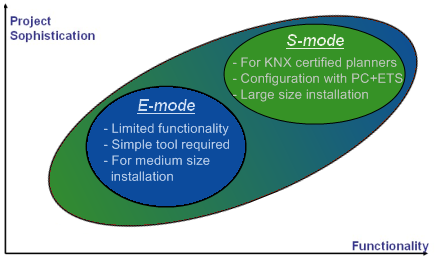
\includegraphics[width=0.9\textwidth]{figures/knx_modes.png}
	\caption{KNX configuration modes \cite{knx}. }
	\label{fig:knx_modes}
\end{figure}
 
 S-mode is intended to be used by experienced KNX installers as it offers full control over the system functions and configurations. The E-mode is targeted to installers with less experience, since components are already pre-programmed with a default array of parameters.
 
To conclude, KNX is capable of resolve most of the problems in the Building Automation field. Features such as the very rigorous certification program for devices from different manufactures is a great way to reduce the heterogeneity in communication between devices.

 
\subsubsection{LonWorks}

LonWorks is an event-triggered control network system \cite{Osorio}, developed by Echelon Corporation \cite{echelon} in 1988. This system uses LonTalk, a communication protocol firstly presented in 1999 as a official ANSI/EIA-709 standard and later as a ISO/International Electrotechnical Commission (IEC) 14908.

LonWorks uses a decentralized peer to peer architecture, where devices are treated as nodes and can communicate with each other by any medium available, using a standard protocol. This node's main component is a Neural Chip which is designed to provide intelligence and network communication capabilities to control devices. In addiction, this nodes have a unique identifier and a set of functionalities and network variables, i.e. all the datapoints needed to nodes communicate directly with each other \cite{Domingues2016}.

Also, the use of a standard network variable types (SNVT), facilitates integration, as it helps in the prevention of errors and simplifies the engineering process \cite{Siemens2013}. 


\subsubsection{DALI}




\subsubsection{EnOcean}
\subsection{\ac{bas} Solutions}

\subsubsection{HCL Technologies \ac{bas}}

\subsubsection{Metasys \ac{bas}}
\subsubsection{Honeywell \ac{bas}}
\subsubsection{Desigo \ac{bas}}
\section{\acf{iot}}



\subsection{\acf{m2m}}
\subsection{\acf{wsan}}
\subsection{Wireless Communication Protocols}
\subsubsection{IEEE 802.15.4}
\subsubsection{6LoWPAN}
\subsubsection{ZigBee}
\subsubsection{\acf{ble}}
\subsubsection{IEEE802.11ah}
\subsubsection{Wireless Communication Protocols Comparison}
\subsection{Interaction Protocols}
\subsubsection{\acf{mqtt}}
\subsubsection{\acf{amqp}}
\subsubsection{\acf{coap}}
\subsubsection{\acf{xmpp}}
\subsubsection{Interaction Protocols Comparison}